\documentclass[my_thesis.tex]{subfiles}

\begin{document}
\chapter{Measures of field line integrability} \label{ch4.diagnostics}

In view to assess the capability of a magnetic equilibrium to confine a plasma, one has to define physics based metrics. In particular, to assess the quality of its magnetic surfaces, it is important to have numerical diagnostics that can determine the topology of a magnetic field line, and how well it confines a plasma. In this chapter, we introduce three different metrics, namely the Greene's residue \citep{Greene1968,Greene1978}, the volume of chaos \citep{Loizu2017}, and the fraction of net parallel diffusion ({\color{red} cite your paper}). These metrics will then be used in different applications: the volume of chaos and the fraction of parallel diffusion to measure the equilibrium $\beta$-limit in a classical stellarator (chapter \ref{ch5.equilibrium_beta_limit}), while objective functions will be constructed using the Greene's residues to optimize stellarator equilibria for good magnetic surfaces (chapter \ref{ch6.optimization}).

\section{Greene's residues} \label{sec.greene residue}
The first metric discussed in this chapter is the Greene's residue  \citep{Greene1968,Greene1978}. The Poincar\'e section of a magnetic equilibrium can be understood as the a map $T(R,Z):\mathbb{R}^2\rightarrow\mathbb{R}^2$, that maps any point $(R_i,Z_i)$ of the $RZ$-plane to another point $(R_{i+1},Z_{i+1})$ after each toroidal transit. One can show that the hamiltonian structure of the magnetic field in a stellarator implies that its Poincar\'e map is a sympleptic twist map \citep{Meiss1992c}. 

Orbits are a sequence of points $\{(R_0,Z_0),\ldots,(R_n,Z_n)\}$, and can form either (i) periodic orbits, which correspond to rational magnetic surfaces, (ii) quasiperiodic orbits, which correspond to irrational surfaces. In case of a resonance, periodic orbits fill a finite volume of the space, \textit{i.e.} a magnetic island is formed. Of particular interests are the O- and X-points of the island chain, thereafter denoted $\mathbf{x}_o$ and $\mathbf{x}_x$ respectively, located at the center and at the edge of the islands. These points are fixed-points of the map $T$, that is $T(\mathbf{x}_{o/x})=\mathbf{x}_{o/x}$. The asymptotic behavior of the orbits close to these points can be studied by looking at the Taylor expansion of the map $T$ around $\mathbf{x}_{o/x}$, 
\begin{equation}
	T(\mathbf{x}_{o/x}+\delta\mathbf{x}) = \mathbf{x}_{o/x} + J_T(\mathbf{x}_{o/x})\delta\mathbf{x},
\end{equation}
where $\delta\mathbf{x}$ is a small displacement from $\mathbf{x}_{o/x}$, and $J_T(\mathbf{x}_{o/x})$ is the jacobian of $T$. As $T$ is sympleptic, $det(J_T)=1$, and the eigenvalues of the jacobian are 
\begin{equation}
	\lambda_{\pm} = \frac{1}{2}\left(Tr(J_T)\pm\sqrt{Tr(J_T)^2 - 4}\right),
\end{equation}
with $Tr(J_T)$ the trace of the jacobian matrix, and, as expected by the sympleptic property of $T$, we have $\lambda_+ = 1/\lambda_-$. The following cases are then possible:
\begin{enumerate}
	\item The trace is smaller than $-2$. The eigenvalues are real, with $\lambda_-<-1$ and $-1<\lambda_+<0$. This corresponds to reflection hyperbolic orbits; the related eigenvectors are tangent to the separatrix at the X-point.
	\item The trace is equal to $-2$. The eigenvalues are then $\lambda_+=\lambda_-=-1$, which corresponds to parabolic orbits.
	\item The trace is greater than $-2$ and smaller than $2$. The eigenvalues are then two complex conjugate values, $\lambda_\pm=e^{\pm 2\pi i \omega}$, with $\omega$ a constant. This corresponds to elliptic orbits that rotates around the O-point.
	\item The trace is equal to $2$. Then $\lambda_+=\lambda_-=1$. In this particular case, the island width is zero and the orbit forms a magnetic surface
	\item The trace is greater than $2$. The eigenvalues are real, with $\lambda_+>1$ and $0<\lambda_-<1$. This corresponds to hyperbolic orbits; the related eigenvectors are tangent to the separatrix at the X-point.
\end{enumerate} 
The Greene's Residue $R$ is defined as
\begin{equation}
	R = \frac{1}{4}\left(2-Tr(J_T)\right).
\end{equation}
For reflection hyperbolic orbits, $R>1$; for elliptic orbits, $0<R<1$; for parabolic orbits, $R=1$; and for magnetic surfaces, $R=0$. We will discuss in chapter \ref{ch6.optimization} how stellarators can be optimized for good magnetic surfaces by minimizing the square of the Greene's residue of some targeted resonances. As an illustrative example, we describe in the next section the standard map and compute its Greene's Residue.

\subsection{Standard map}
The standard map is a canonical example of a 2-dimensional non-linear map. It is defined as $(x',y')= T(x,y)$, with
\begin{align}
	y' &= y - \frac{k}{2\pi}\sin(2\pi x) \label{eq.std_map_y}\\
	x' &= x + y', \label{eq.std_map_x}
\end{align} 
with $k$ a parameter, that controls the "strength" of the non-linearity in the system. We plot the phase space of the standard map for four different values of $k$ in Figure \ref{fig.std map phase space}. 

\begin{figure}
	\centering
	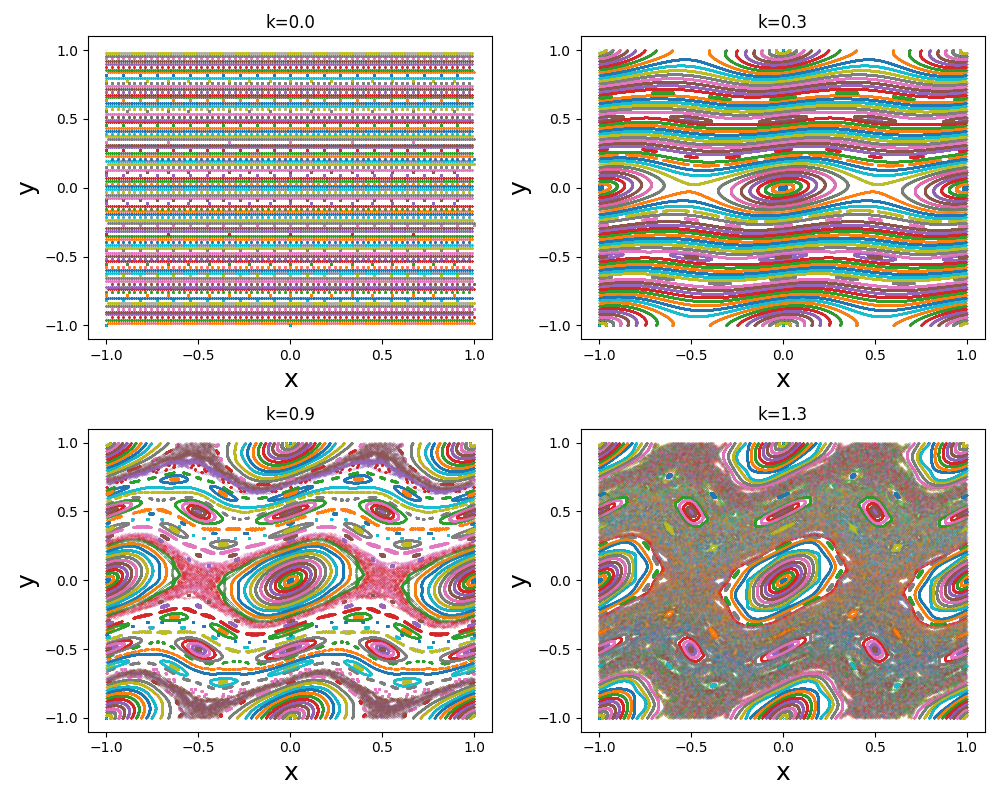
\includegraphics[width=\linewidth]{images/std_map_phase_space.png}
	\caption{Phase space of the standard map for four different values of $k$, as described by Eqs.(\ref{eq.std_map_y})-(\ref{eq.std_map_x}).}
	\label{fig.std map phase space}
\end{figure}

The points $\mathbf{x}_o=(x=0,y=0)$ and $\mathbf{x}_x=(x=1/2,y=0)$ are both fixed points of the standard map, as $T(\mathbf{x}_{o/x})=\mathbf{x}_{o/x}$. We study the behavior of the orbits close to these points by looking at the jacobian of $T$,
\begin{equation}
	J_T = \begin{pmatrix}
		1-k\cos(2\pi x) & 1 \\
		-k\cos(2\pi x) & 1
	\end{pmatrix}.
\end{equation}
We notice that the linearized map is sympleptic, since $det(J_T)=1$, which is a necessary and sufficient condition for linear maps to be sympleptic in 2D. The eigenvalues of $J_T$ are then
\begin{equation}
	\lambda_\pm = \frac{1}{2}\left(2-k\cos(2\pi x) \pm \sqrt{(2-k\cos(2\pi x))^2-4}\right),
\end{equation}
and the Greene's residue is
\begin{equation}
	R = \frac{k}{4}\cos(2\pi x).
\end{equation}
At $\mathbf{x}_o$, the Greene's residue is zero if and only if $k=0$, which, as seen on top left panel of Figure \ref{fig.std map phase space}, corresponds to a phase space without island. For $0<k<4$, the orbits around the $\mathbf{x}_o$ fixed points are elliptic, and corresponds to the existence of a magnetic island. Finally, for $k>4$, the orbits become hyperbolic. For such large values of $k$ however, the phase space is mostly filled with chaotic orbits, making any observation difficult. Regarding the $\mathbf{x}_x$ fixed-point, it is again zero if and only if $k=0$. For any values of $k>0$ however, the residue is smaller than $0$. Orbits close to the fixed point are hyperbolic, which correspond to an X-point at $\mathbf{x}_o$.


The Greene's residues are a great measure to assess whether or not a rational surface is resonant and magnetic island are present. However, this measure is a local measure --- as it will be discussed in chapter \ref{ch6.optimization}, this can be a limitation when performing stellarator optimization. In addition, the Greene's residue gives no information on the impact of the field line topology on the plasma confinement.





\section{Volume of chaos} \label{sec.volume chaos}
One approach to discriminate between a chaotic field line and other magnetic field line topologies is to evaluate the fractal dimension $D$ of the field line Poincar\'e section, for example using a box-counting algorithm \citep{Meiss1992c}. Assume that a field line Poincar\'e section is provided as a set $S$ of $N$ points in the $RZ$-plane, $S\equiv\{(R_i,Z_i)\}_{i=\{1,\ldots,N\}}$. We split the $RZ$-plane in a grid made of squares of dimension $L\times L$ and count the number $N$ of grid element $\Omega_{ij}$ that contains at least one point from the field line,
\begin{equation}
    N(L) = \left|\{\Omega_{ij}|S\cap\Omega_{ij}\neq\emptyset\}\right|,
\end{equation}
where $|\cdot|$ denotes the cardinality. The box-counting dimension (or Hausdorff dimension) is then given by
\begin{equation}
    D = \lim_{L\rightarrow 0} \frac{\log N(L)}{\log L}.
\end{equation}
An almost binary behavior is then observed: either a magnetic field line stays on a magnetic surface whose Poincar\'e section is a one-dimensional object, $D=1$, or the magnetic field line has a fractal dimension $D>D_{crit}$, with $1<D_{crit}<2$. In our case, we observe that $D_{crit}=1.3$ can be used to differentiate between magnetic surfaces and chaos.
\citet{Loizu2017} proposed to evaluate the volume occupied by chaotic field lines with
\begin{equation}
	V_{chaos} = V_{total} \sum_{i=1}^{N_{lines}} \frac{(\psi_{t,i}-\psi_{t,i-1})}{\psi_a}\mathcal{H}(D_i-D_{crit}), \label{eq.volume chaos}
\end{equation}
where $N_{lines}$ is the number of considered field lines, $D_i$ is the fractal dimension of the $i^{\text{th}}$ line, $\mathcal{H}$ is the Heaviside function, $V_{total}$ is the total plasma volume, and $\psi_{t,i}-\psi_{t,i-1}$ measures the enclosed toroidal flux between field lines $i$ and $i-1$. As an illustration of the volume of chaos, it can be evaluated for the standard map defined in Eqs.(\ref{eq.std_map_y})-(\ref{eq.std_map_x}) as a function of the parameter $k$ for different values of $D_{crit}$ (see Figure \ref{fig. std_map_v_chaos}). The same trend is observed for the three considered values of $D_{crit}$: for low values of $k$, the volume of chaos is zero; a critical value of $k$, between $0.5$ and $0.8$, marks the emergence of chaotic orbits; for large values of $k$, the normalized volume of chaos tends to $0.8$ --- the remaining non chaotic orbits are those close to O-points inside islands. This work was part of a summer internship of H. Arbez at the Swiss Plasma Center in 2021 {\color{red} add citation to internal report}. 
\begin{figure}
	\centering
	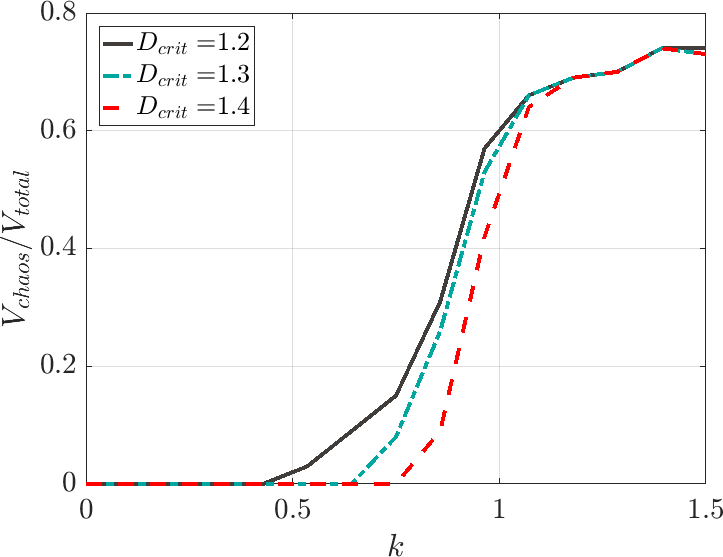
\includegraphics[width=.7\linewidth]{images/std_map_vchaos.png}
	\caption{Normalized volume of chaos in the standard map as a function of $k$ for different values of $D_{crit}$ {\color{red} add citation to internal report}.}
	\label{fig. std_map_v_chaos}
\end{figure}

When applied to Poincar\'e maps of magnetic field lines, the volume of chaos is a global measure of the amount of chaotic field lines in the system, in opposition to the Greene's residue, which was a local measure of the field line topology (see section \ref{sec.greene residue}). Both measures, however, don't provide information on the plasma confinement properties of the magnetic equilibrium. Indeed, structures present in chaotic magnetic field lines and magnetic islands can, potentially, support temperature and density gradients \citep{Hudson2008,hudsonAreGhostSurfaces2009}. Considering all magnetic islands and chaotic field lines as detrimental for confinement can thus be a pessimistic diagnostic of the confinement properties of the magnetic equilibrium. In the next section, we propose an alternative measure, specific to the Poincar\'e map of stellarator magnetic fields, that counts the fraction of resonances in the equilibrium that are important sources of transport.

\section{Fraction of net parallel diffusion}\label{sec.fraction parallel diffusion}
We discuss an alternative measure to the volume of chaos to determine if the destruction of magnetic surfaces significantly impacts the radial transport. Here the parallel and perpendicular direction are defined as the direction along and across the magnetic field respectively, and the radial  direction $r$ as the direction perpendicular to isotherms, $\nabla T\times\nabla r=0$, with $T$ the temperature. In recent work, \citet{paulHeatConductionIrregular2022} discussed the properties of the anisotropic heat diffusion equation, $\nabla\cdot(\kappa_\parallel T + \kappa_\perp T)=0$, where $\kappa_\parallel$ and $\kappa_\perp$ are the parallel and perpendicular heat conductivities. In particular, \citeauthor{paulHeatConductionIrregular2022} demonstrated that, under the assumption that $\boldsymbol{\kappa}$ and $\nabla\cdot\boldsymbol{\kappa}$ are analytical, isotherms are topologically constrained to be toroidal surfaces --- this forbids isotherms to align with the magnetic field in regions occupied by magnetic islands and magnetic field line chaos. Motivated by comparing the local parallel diffusion to the local perpendicular diffusion, \citeauthor{paulHeatConductionIrregular2022} introduced the \emph{volume of effective parallel diffusion}, which is the volume of plasma where the parallel heat transport dominates perpendicular heat transport,
\begin{equation}
V_{PD} = \frac{1}{V_{total}} \int_{V_{total}}\mathcal{H}(\kappa_\parallel|\nabla_\parallel T|^2-\kappa_\perp|\nabla_\perp T|^2) d\mathbf{x}^3, \label{eq.paul_volume_effective_diffusion}
\end{equation}
where the parallel and perpendicular gradients are defined as $\nabla_\parallel=\mathbf{B}(\mathbf{B}\cdot\nabla) / B^2$ and $\nabla_\perp=\nabla-\nabla_\parallel$ respectively. In regions occupied by magnetic islands and magnetic field line chaos, the constraint on the isotherms topology implies that the magnetic field has a non-zero radial component, thus $\nabla_\parallel T> 0$. Depending on the ratio $\kappa_\parallel / \kappa_\perp$, the volume of effective parallel diffusion can then be greater than zero. On the contrary, in regions occupied by magnetic surfaces, isotherms largely coincide with magnetic surfaces, which means that $\nabla_\parallel T$ is negligible, and consequently the volume $\mathcal{V}_{PD}$ is zero. Leveraging these properties, we can define the equilibrium $\beta$-limit as the $\beta$ above which $V_{PD}>0$.

To determine the equilibrium $\beta$-limit, it is only required to determine if $V_{PD}$ is zero or not; its absolute value is irrelevant. We thus construct a proxy function for $V_{PD}$ that does not depend on the temperature profile, but only on the magnetic field. We start by noticing that the Heaviside function in Eq.(\ref{eq.paul_volume_effective_diffusion}) is greater than zero when $\kappa_\parallel|\nabla_\parallel T|^2\ge \kappa_\perp|\nabla_\perp T |^2$. As we expect the radial magnetic field to be small in comparison to the total magnetic field, $B_r\ll B$, we can write $\nabla_\parallel T\sim \nabla T\ B_r /B$, and $\nabla_\perp T\sim \nabla T$. The volume of effective parallel diffusion is then greater than zero if there is a finite volume where
\begin{equation}
	\left(\frac{B_r}{B}\right)^2  \ge  \frac{\kappa_\perp}{\kappa_\parallel} \equiv \left(\frac{B_{r,crit}}{B}\right)^2.\label{eq.bcrit_estimate}
\end{equation}
Considering the electron heat transport as a figure of merit for the confinement properties of the equilibrium, and using the Spitzer-H\"arm conductivity for $\kappa_{\parallel,e}$ \citep{s.i.braginskiiTransportProcessesPlasma1965}, we get
\begin{equation}
	\left(\frac{ B_{r,crit}}{B}\right)^2 =  5.2\cdot 10^{-22}\frac{n_e\log\Lambda \  \chi_{\perp,e}}{T_e^{5/2}},
\end{equation}
where $\log\Lambda$ is the Coulomb logarithm, and typically $\chi_{\perp,e}=\kappa_{\perp,e}/n_e\sim 1 \text{m}^2\text{s}^{-1}$. Here everything is to be expressed in SI units except $T_e$, which is in $eV$. For temperatures and densities between $1$ to $10$ keV and $10^{19}$ to $10^{20}\text{m}^{-3}$ respectively, $ B_{r,crit}/B$ ranges from $10^{-6}$ to $10^{-4}$. For example using typical values for W7-X high performance experiments \citep{klingerOverviewFirstWendelstein2019}, \textit{i.e.} $n_e=4\cdot10^{19}\text{m}^{-3}$, $T_e=5\ \text{keV}$, we obtain a critical normalized radial magnetic field of $ B_{r,crit}/B\sim 10^{-5}$. As a side note, we remark that the criterion (\ref{eq.bcrit_estimate}) can also be derived by considering the radial heat diffusion equation for electrons, $q_r = -\kappa_{\perp,e} (\nabla_\perp T_e)_r - \kappa_{\parallel,e} (\nabla_\parallel T_e)_r \sim -\kappa_{\perp,e} dT_e/dr -\kappa_{\parallel,e} dT_e/dr B_r^2/B^2$. Magnetic islands and chaos play then an important role in setting the local heat radial transport when the second term on the right hand side of the heat diffusion equation is larger than the first one, which occurs when $B_r^2/B^2\ge \kappa_\perp/\kappa_\parallel$, recovering equation (\ref{eq.bcrit_estimate}).

The volume of effective parallel diffusion can thus be written using the criterion (\ref{eq.bcrit_estimate}),
\begin{equation}
	V_{PD} \sim \frac{1}{V_{total}} \int_{V_{total}}\mathcal{H}\left(\left[\frac{ B_{r}}{B}\right]^2-\left[\frac{ B_{r,crit}}{B}\right]^2\right) d\mathbf{x}^3.
\end{equation}
This measure is however unpractical for the purpose of this paper, as it would require to evaluate the radial magnetic field everywhere in the plasma. Instead, the radial magnetic field is evaluated where it is expected to be the largest, \textit{i.e.} on a selected number of rational surfaces. We then construct \emph{the fraction of parallel diffusion},
\begin{equation}
	f_{PD} = \frac{1}{N_{res}}\sum_{i=1}^{N_{res}} \mathcal{H}\left(\left[\frac{B_{r}}{B}\right]^2-\left[\frac{B_{r,crit}}{B}\right]^2\right), \label{eq.def metric}
\end{equation}
where $N_{res}$ is the number of considered resonances, and the algorithm used to evaluate the radial magnetic field $B_r$ from SPEC equilibria is described in section \ref{sec. measure b r}. The fraction of effective parallel diffusion is then the fraction of resonances in the plasma that contribute to the transport, \textit{i.e.} the fraction of resonances over which the diffusion due to parallel dynamics dominates. Note that $f_{PD}\neq V_{PD}$, but if $f_{PD}=0$, we can expect $\mathcal{V}_{PD}$ to be zero, and the opposite is true as well. The fraction of parallel diffusion can then be used as a proxy function to determine if the volume of parallel diffusion is zero or not. The chaotic equilibrium $\beta$-limit, $\beta^{chaos}_{lim}$, is obtained by taking the value of $\beta$ above which $f_{PD}>0$. 


% The metric $f_{PD}$ has the property to be non-zero whenever a resonance in the plasma contributes to the radial transport at least as much as the turbulent transport, according to the equation (\ref{eq.bcrit_estimate}). 




\subsection{Measure of the radial magnetic field} \label{sec. measure b r}
To evaluate the radial electric field $ B_r$, it is useful to construct a general set of coordinates, such as quadratic flux minimizing (QFM) surfaces \citep{dewarAlmostInvariantManifolds1994, hudsonAlmostinvariantSurfacesMagnetic1996, hudsonConstructionIntegrableField1998}, or ghost surfaces \citep{hudsonAreGhostSurfaces2009}, which have been shown to coincide with isotherms \citep{Hudson2008}. We construct QFM surfaces  using the pyoculus package\footnote{\url{https://github.com/zhisong/pyoculus}}. These surfaces, thereafter named $\Gamma_{mn}$, are smooth toroidal surfaces that pass through the X- and O- points of the island chain corresponding to the $\iotabar=n/m$ rational resonant surface, and are constructed by finding the surfaces $\Gamma_{mn}$ minimizing the weighted quadratic flux $\int_{\Gamma_{mn}} w (B\cdot\mathbf{n})^2 dS$, where the weight $w$ is cleverly chosen such that the underlying Euler-Lagrange equation has non-singular solutions. Some examples of QFM surfaces are plotted in Figure \ref{fig.qfms_example}. The radial coordinate $r$ is then defined as the direction perpendicular to the QFM surfaces.

\begin{figure}
	\centering
	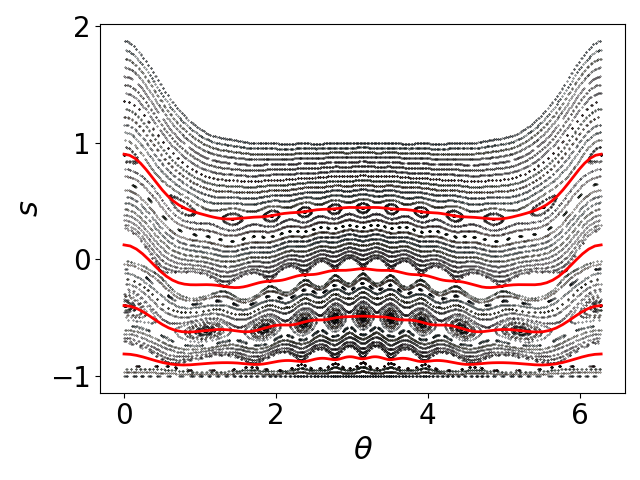
\includegraphics[width=.75\linewidth]{images/QFMS_example.png}
	\caption{Black: Poincar\'e plot with magnetic surfaces and magnetic islands. Red: QFM surface $r=\text{const}$. The coordinate $s$ is a radial-like coordinate.}
	\label{fig.qfms_example}
\end{figure}

We can now measure the radial component of the magnetic field at each resonant surface $\iotabar=n/m$. We start by identifying all potential resonances $(m,n)\in\mathbb{N}$ in each volume $\mathcal{V}_l$, such that (i) $n/m$ is within the rotational transform extrema in the volume, and (ii) $n$ is a multiple of the number of field periods. We construct QFM surfaces $\Gamma_{mn}$ for each of the identified resonances $\iotabar=n/m$. The magnetic field perpendicular to the QFM surface, $ B_r$, is obtained by projecting  the magnetic field on their normal direction, and the magnetic field resonant harmonic, $ B_{r,mn}$ is obtained after a standard Fourier transform of $ B_r$. We expect the Fourier spectrum of $ B_r$ to be largely dominated by the $(m,n)$ harmonic, and assume $ B_r\approx B_{r,mn}$ to filter out numerical noise that may be generated by the QFM surface construction.

Only resonances with large radial magnetic field will significantly participate to the radial transport. Since the magnetic field harmonics $B_{mn}$ are expected to decrease exponentially with the square of their mode numbers $m$ and $n$, \textit{i.e.} $B_{mn}\sim exp(-m^2-n^2)$, we can discard resonances with large poloidal and toroidal mode number and study only harmonics with mode number smaller than a given resolution, $m\leq M_{res}$ and $n\leq N_{res}$. In this paper, we set $M_{res}=25$ and $N_{res}=10$. 


\end{document}